\documentclass[tikz]{standalone}
\usepackage{tikz,amsmath}
\usetikzlibrary{shapes}
\begin{document}
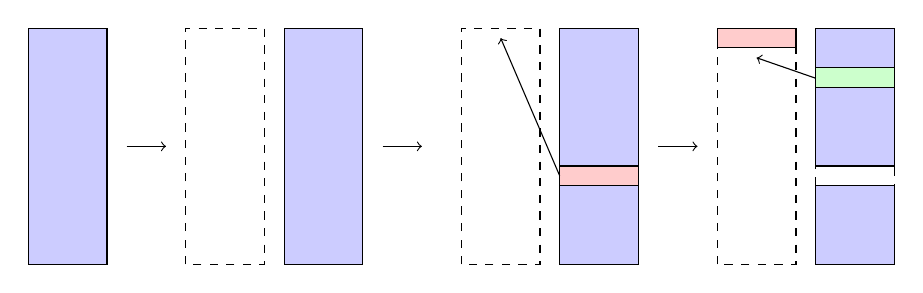
\begin{tikzpicture}
    \draw [fill = blue!20] (0,0) -- (0,3) -- (1,3) -- (1,0) -- cycle;

    \draw [->] (1.25,1.5) -- (1.75,1.5);

    \draw [dashed] (2,0) -- (2,3) -- (3,3) -- (3,0) -- cycle;
    \draw [fill = blue!20] (3.25,0) -- (3.25,3) -- (4.25,3) -- (4.25,0) -- cycle;

    \draw [->] (4.5,1.5) -- (5,1.5);

    \draw [dashed] (5.5,0) -- (5.5,3) -- (6.5,3) -- (6.5,0) -- cycle;
    \draw [fill = blue!20] (6.75,0) -- (6.75,3) -- (7.75,3) -- (7.75,0) -- cycle;
    \draw [fill = red!20] (6.75,1) -- (6.75,1.25) -- (7.75,1.25) -- (7.75,1) -- cycle;
    \draw [->] (6.75,1.125) -- (6,2.875);

    \draw [->] (8,1.5) -- (8.5,1.5);

    \draw [dashed] (8.75,0) -- (8.75,3) -- (9.75,3) -- (9.75,0) -- cycle;
    \draw [fill = blue!20] (10,0) -- (10,1) -- (11,1) -- (11,0) -- cycle;
    \draw [dashed] (10,1) -- (10,1.25) -- (11,1.25) -- (11,1) -- cycle;
    \draw [fill = blue!20] (10,1.25) -- (10,3) -- (11,3) -- (11,1.25) -- cycle;
    \draw [fill=red!20] (8.75,3) -- (8.75,2.75) -- (9.75,2.75) -- (9.75,3) -- cycle;
    \draw [fill=green!20] (10,2.25) -- (10,2.5) -- (11,2.5) -- (11,2.25) -- cycle;
    \draw [->] (10,2.365) -- (9.25,2.625);
\end{tikzpicture}
\end{document}
